\section{Lokale Modelle}
Für das Ausführen von Modellen zum Testen werden in dieser Arbeit zwei Techniken angewandt. Zum einen mittels Ollama Framework, das mit einer Web-GUI erweitert werden kann, zum anderen durch Dateien die beispielsweise mit dem Python Framework Langchain abgefragt werden können.\vspace{0.2cm}

Die Modelle werden auf einem Debian 12 Server mit 32 GB RAM und einem 16 Kernprozessor ausgeführt. Demnach können nur kleine Modelle lokal getestet werden.\vspace{0.2cm}

\subsection{Modellbereitstellung mit Ollama}
Für das Testen der lokalen Modelle wird das Ollama Framework angewandt. Dies ermöglicht eine neben einer Benutzeroberfläche im Browser eine Anbindung an einer API. Diese lässt sich beispielsweise mittels Python abfragen. Auf dieser Weise lassen sich Modelle von der \href{https://ollama.com/search}{Ollama Modell} Seite testen.\vspace{0.2cm}

Dazu wird Ollama auf dem Server installiert und konfiguriert, siehe Anhang \ref{sec:install_config_ollama_local}. Nach dem Download stehen die Modelle zur Verfügung und es können Interaktionen mit dem Modell erfolgen. Zusätzlich kann ein grafisches Tool zum Testen installiert werden. Hier wird Open WebUI eingesetzt und auf dem Ollama-Server installiert, welches mittels Webbrowser geöffnet wird. Nach der Installation, wie in Anhang \ref{sec:open_webui} beschrieben, ist das Tool einsatzbereit und im Netzwerk erreichbar, unter http://<<server-ip>>:<<webui-port>>.

\subsection{Modellbereitstellung als Datei}
Eine zweite Methode zur Bereitstellung von Modellen ist die direkte Nutzung mittels Programmiersprache. In dieser Arbeit wird Python verwendet. Hierbei ist die Nutzung von Hugging Face Modelle vorgesehen. Kontrolle der Daten (Modelle und Datensätze) die von \textit{Hugging Face} geladen wurden. Diese Modelle lassen sich mit dem Python Framework \href{https://pypi.org/project/langchain/}{Longchain} orchestrieren.\vspace{0.2cm}

Zunächst lädt man die Modelle von Hugging Face herunter und lokal abgespeichert. Ein Beispiel für ein Download-Skript ist in Anhang \ref{lst:download_hugging_face_model} zu sehen. Auch hier ist die Speichergröße zu beachten.

\begin{verbatim}
	huggingface-cli scan-cache
	huggingface-cli remove-cache
\end{verbatim}

\subsection{Orchestrierung von Modellen}
Die Orchestrierung der Modelle erfolgt mithilfe des Python-Frameworks Longchain. Hierbei werden an die Modelle verschiedene Anforderungen gestellt. Zum einen müssen die Modelle Code generieren, zum anderen ist die Anforderung Text zu erstellen oder zu überarbeiten. Die Abbildung \ref{img:orchestration_llms} zeigt schematisch den Aufbau der orchestrierten Modelle. Der Textfilter sucht in der Ausgabe des ersten Modells den Prompt und eliminiert die Anweisungen und Erklärungen.

\begin{figure}[!ht]
	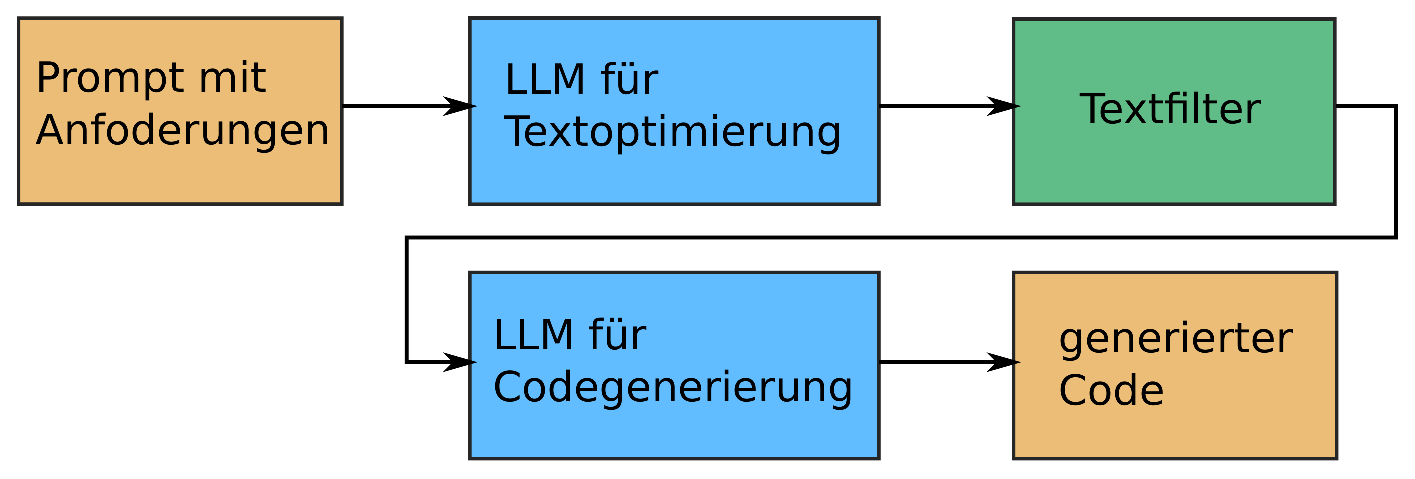
\includegraphics[width=0.8\textwidth]{content/chapter_implementation/images/orchestrierung_llms.eps}
	\centering
	\caption{Orchestrierte LLM's für die Codegenerierung}
	\label{img:orchestration_llms}
\end{figure}

\section{Online Modelle}
Text.

\section{Benchmark Codeevaluation}\label{sec:benchmark_evaluation}

\textbf{Umsetzung der pass@k Metric}\vspace{0.2cm}

In Python steht, hierfür die Bibliothek \textit{pass\_at\_k} zur Verfügung. Der PHP Code wurde auf einen Debian 11 mit PHP in der Version 8.2.26 evaluiert.

\begin{lstlisting}[language=Python,label=lst:pass_at_k,caption={Berechnung der pass@k Metrik in Python}]
	def custom_pass_at_k(n: int, c: int, k: int) -> float:
	"""
	:param n (int): numbers of total samples.
	:param c (int): number of currect samples.
	:param k (int): number of consider samples.
	"""
	if n - c < k:
	return 1.0
	return 1.0 - np.prod(1.0 - k / np.arange(n - c + 1, n + 1))
\end{lstlisting}


\section{Codeevaluation mit Frameworks}
Neben dem bekannten Evaluationen mit beispielsweise dem HumanEval Benchmark, wird hier eine weitere Testmethodik überprüft, die mit verschiedenen Validierungstools der jeweiligen Programmiersprache ausgeführt wird. Für die Erstellung der Abfragen wird das Python-Skript verwendet, was schon im Kapitel \ref{sec:benchmark_evaluation} vorgestellt wurde.

\subsection{PHP Codeevaluation}
Der Test wird bei den erweiterten Problemen durchgeführt und beginnt mit den Unit-Tests die mit \textit{PHPUnit} durchgeführt werden. Im Anschluss wird \textit{PHPMetrics} ausgeführt. Hierbei wird geprüft, ob die Codekomplexität und Wartbarkeit überprüft. Sind diese Tests bestanden, wird der Code noch gegen eine \textit{SonarQube} Server validiert. Die Ausführung der Tests wird mithilfe eines Python-Skripts durchgeführt. Es wird eine PHP Datei erstellt, die mit den Frameworks geprüft wird.

\subsection{JavaScript Codeevaluation}
Text.

%\section{Online Modelle}
% Eigenen KI Server \href{https://www.computerweekly.com/de/ratgeber/Einen-KI-Server-mit-Ollama-und-Open-WebUI-einrichte}{Computer Weekly}
% Orchestrierung mit Python \href{https://pypi.org/project/multillm/}{multillm-Projekt}
% LangChain Library \href{https://python.langchain.com/api_reference/ollama/chat_models/langchain_ollama.chat_models.ChatOllama.html}{Example}
% \href{https://pypi.org/project/langchain-ollama/}{Python lib langchain-ollama}
% YouTube \href{https://www.youtube.com/@AICodeKing}{AICodeKing}
